%----------------------------------------------------------------------------
\chapter{Abstraction analysis on \cfa}
\label{sec:cfa}
%----------------------------------------------------------------------------


%----------------------------------------------------------------------------
\section{program representation}
%---------------------------------------------------------------------------- 

A program most commonly is represented by a source code. Example: an average counter function in c

\begin{lstlisting}[language=C,breaklines=true]
int average(int a, int b){
int avg;
avg=(a+b)/2;
return avg;
}
\end{lstlisting}

There are many different type of code languages, making a static analyzer for all, would be hard and unnecessarily time-consuming. 

%----------------------------------------------------------------------------
\section{\cfa (CFA)}
\label{sec:cfaleiras}
%---------------------------------------------------------------------------- 
CFA can describe the programs as graphs, where edges are annotated with program statements. The Theta framework \hyperref[sec:ref]{[4]} provides a representation of a CFA formalism.

A CFA is a directed graph with
 
\begin{itemize}
	\item variables,
	\item locations, with dedicated initial, final and error locations,
	\item edges between locations, labeled with statements over the variables.
\end{itemize}

\begin{enumerate}
	\item Assume: check if a condition is true for the variables
	\item Assign: assign a concrete value to a variable
	\item Havoc: assign a random value to a 
	\item Skip: no action
\end{enumerate}

\label{fig:simpleC}This simple C code translates to 5 location:
\begin{lstlisting}[language=C,breaklines=true]
//Loc1
int a=1;
//Loc2
if(a!=1){
	//errorLOC
}
else {
//Loc3
	printf("%d", a);
}
//Loc4
\end{lstlisting}

The edges are the program statements. For example from Loc1 to Loc2 an assign statement which set a variable to 1, and from Loc2 to Loc3 is an assume statement (!(a!=1)).

Analysis is usually made for reachability of the error state.

%----------------------------------------------------------------------------
\section{Abstraction analysis algorithm for CFA}
\label{sec:cfaalgorithm}
%---------------------------------------------------------------------------- 

\begin{figure} [!ht]
	\centering
	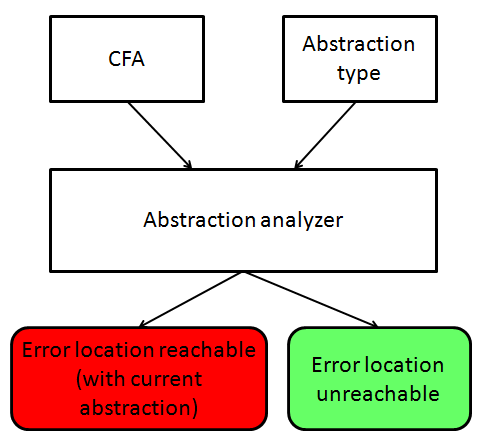
\includegraphics[width=100mm, keepaspectratio]{figures/abstractanalyzer.png}
	\caption{\label{fig:absanalyzer} Abstraction analysis model}
\end{figure}

The CFA provides only one error state. This is not a problem since if there is more, then a simple abstraction can make one error state that contains all.

$\forall i$ $S_{P}^{i} \in $ Error states $S_{P}^{'error}=\cup S_{P}^{i}$

Label: representation of the Program. (in section \hyperref[sec:saai]{SAAI} these were the states of the program  $S_{P}^{i}$). Usually it will be a representation of the CFA's variables.

Every abstraction type need to have its own Label type. For example in case of sign abstraction a label type would be a (-), (+) or (-+) assigned to every variable (meaning: it can only be minus, it can only be positive, it can be both).

The possible trajectories are represented in the CFA by iterations of the CFA graph. So the problem of reaching the error states, in CFA means that there is no valid path from the initial location to the error location. Valid means that every edge in the path is a possible step.

For example a possible trajectory in \hyperref[fig:simpleC]{the code from the previous section} is Loc1, Loc2, Loc3, Loc4 (this is the only possible trajectory since Loc2 -> errorLoc edge is an impossible step (a is 1)).

The validation test on an edge is only possible if we put labels to the locations and from the label it is possible to decide that an edge is valid or not. Note: the edge can only be invalid if it has an assume statement
For example if we use sign abstraction and on LocationA we have a label that $var=(+)$ than we can decide wether edge LocationA -> LocationB is valid or not. For example $var>0$ is valid, but $var<0$ is not.

Apply the statement:
If an edge is valid, than we put a new label to the target location (the target of the edge) according to the statement on the edge.
It has two different cases; if the target does not have a label, that means we have reached it for the first time. In this case from the source's label and the edge's statement, we need to be able, to decide the targets label. This is actually depending on the partition tactic (\hyperref[sec:partition]{see Partition in previous chapter}).
If the target already has a label we need to take it into account. This is depending on the widening tactic (\hyperref[sec:widening]{see Widening in previous chapter}).  

Discovered locations:
All the locations that have been reached, and therefore have a label.

Discovered mapping:
Every discovered location mapped with its label. When we apply a statement we modify the Discovered mapping (change the label for one location or add a completely new location).

Modifying edge:
All the outgoing edges from those locations whose label have been modified from the previous Discovered mapping

Fixpoint:
The point where the Discovered mapping can not be changed anymore. So there is no more modifying edges. Note: this is equivalent to: the previous Discovered mapping is the same as the current one (if we applied all the modifying edges from the previous discovered mapping).

Initial step: we put a label on the initial location (it is given in the CFA). Therefore every label type should have an initial label. It represents the program state, where we do not know anything, for example in sign abstraction every variable should be assigned to (+-), since both (+) and (-) can be true.

Iteration:
Let there be a set of discovered locations $D(L)$, and a discovered mapping $M(Loc, Label)^{n}$ and the error location is $ELOC$.
If $ELOC \in D(L)$ we can stop the iteration we reached the error location.
Otherwise If $M(Loc, Label)^{n-1} == M(Loc, Label)^{n}$ we can stop there are no more modifying edges we reached a fixpoint therefore the error location is not reachable.
If $M(Loc, Label)^{n-1} != M(Loc, Label)^{n}$ than we get all the modifying edges from $M(Loc, Label)$ and apply all of the statements in the modifying edges.
If one location is modified by more than one statement we add these labels together, for example in sign abstraction $var=(-)$ and $var=(+)$ are the two modifying statements, then we put $var=(-+)$. So labels should also support this operation. 

If a location is reached and labeled, than its new label can only be less specific.
For example in sign abstraction LocA has a $var=(+-)$ label than if there is a statement which assigns $var=(+)$ it can not narrow down LocA's label as in LocA (-) is already possible (in at least one trajectory).

Partitioning and widening can differ according to what type of abstraction are we using.

\begin{figure} [!ht]
	\centering
	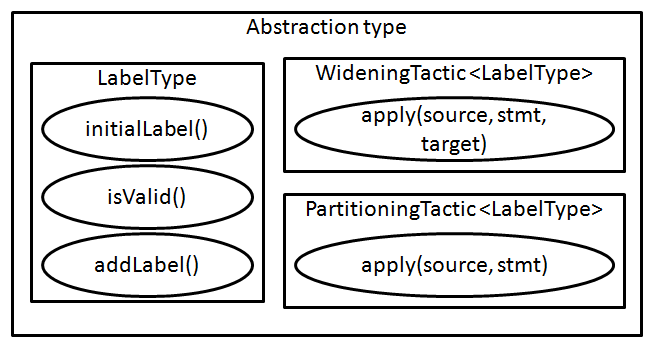
\includegraphics[width=150mm, keepaspectratio]{figures/abstractiontype.png}
	\caption{\label{fig:abstype} The structure of an Abstraction type}
\end{figure}








